\documentclass[10pt]{article}

\usepackage[a4paper,margin=1.3cm,top=1.0cm,bottom=1.0cm]{geometry}
\usepackage[T1]{fontenc}
\usepackage[utf8]{inputenc}
\usepackage{lmodern}
\usepackage{microtype}
\usepackage{graphicx}
\usepackage{xcolor}
\usepackage{enumitem}
\usepackage{titlesec}
\usepackage{pdflscape}
\usepackage{tikz}
\usetikzlibrary{arrows.meta, positioning, fit, backgrounds, calc}

\usepackage[colorlinks=true, linkcolor=blue, urlcolor=blue, citecolor=blue,
            pdftitle={CbcSolver Architecture Overview},
            pdfauthor={Cbc / coin-or}]{hyperref}

\setlength{\parindent}{0pt}
\setlength{\parskip}{1.5pt}

\titlespacing*{\section}{0pt}{3pt}{1pt}
\titlespacing*{\subsection}{0pt}{2pt}{1pt}
\renewcommand{\thesection}{\arabic{section}}
\setlist{itemsep=0.5pt, topsep=1pt, parsep=0pt}

% ---- GitHub source link helpers (coin-or/Cbc, next branch) ----
\newcommand{\GHBASE}{https://github.com/coin-or/Cbc/blob/next/src}
\newcommand{\ghc}[2]{\href{\GHBASE/CbcSolver.cpp\#L#1}{#2}}
\newcommand{\ghh}[2]{\href{\GHBASE/CbcSolver.hpp\#L#1}{#2}}

% ---- Colour palette (shared with diagram page) ----
\definecolor{capi}{RGB}{31,86,161}       % public API - blue
\definecolor{cbab}{RGB}{198,90,16}       % BAB pipeline - burnt orange
\definecolor{cother}{RGB}{47,125,54}     % other run() actions - green
\definecolor{cdata}{RGB}{90,90,90}       % data / state - grey
\definecolor{cutil}{RGB}{116,66,158}     % misc utility helpers - purple

\newcommand{\swatch}[1]{\tikz[baseline=-0.6ex]{\fill[#1] (0,0) rectangle (0.32,0.32);}}

\begin{document}
\pagestyle{empty}
\sloppy

\begin{center}
  {\Large\bfseries CbcSolver: Class Architecture Overview}\\[1pt]
  {\small \texttt{coin-or/Cbc} --- \texttt{next} branch --- \texttt{src/CbcSolver.hpp} / \texttt{src/CbcSolver.cpp}}
\end{center}
\vspace{1pt}

\section*{What is \texttt{CbcSolver}?}
\ghh{90}{\texttt{CbcSolver}} is the top-level driver class for the Cbc MIP solver executable and library
entry point, encapsulating the entire solve pipeline --- parameter initialization, command-queue
parsing, LP relaxation solves, preprocessing, cut/heuristic configuration, branch-and-bound search,
post-processing, and result reporting --- that used to live in the free functions \texttt{CbcMain0}/\texttt{CbcMain1},
now thin backward-compatible wrappers delegating to \ghc{2637}{\texttt{initialize()}} and \ghc{9963}{\texttt{run()}}.

Historically, \ghc{9963}{\texttt{CbcSolver::run()}} was a single $\sim$14{,}000-line function built around one
giant \texttt{switch} on the current command. A series of refactors (most recently: removing dead
\texttt{\#ifndef JJF\_ONE} / \texttt{\#if~0} blocks, splitting the branch-and-bound \texttt{case} into six
cooperating private methods, and deleting the legacy hard-coded \texttt{-miplib}/\texttt{-unitTest}
self-test harness) progressively extracted coherent phases into named methods listed below, while
\texttt{run()} itself was reduced to a slim command dispatcher. Local variables that needed to survive
across these phases were promoted to \texttt{private} data members (see \S\ref{sec:state}).

\footnotesize
\section{Public API surface}
\begin{itemize}[leftmargin=1.4em, itemsep=1pt]
  \item \textbf{\swatch{capi} Construction \& lifecycle:} default / from-solver / from-model / copy
    constructors, \texttt{operator=}, destructor (\ghc{1927}{lines 1927--2341}); \ghc{2637}{\texttt{initialize()}}
    sets up signal handlers and default parameters (replaces \texttt{CbcMain0}).
  \item \textbf{\swatch{capi} High-level solve:} \ghc{2783}{\texttt{solve(file)}}, \ghc{2801}{\texttt{importModel(file)}},
    \ghc{2817}{\texttt{solveLp(method)}} --- convenience one-call wrappers that chain
    \texttt{initialize()} + \texttt{run()} or solve the LP relaxation directly.
  \item \textbf{\swatch{capi} Result accessors:} \texttt{status()}, \texttt{objectiveValue()}, \texttt{bestBound()},
    \texttt{bestSolution()}, \texttt{numCols()}, \texttt{nodeCount()}, \texttt{iterationCount()}, \texttt{hasSolution()}
    --- valid after \texttt{solve()}/\texttt{run()} returns.
  \item \textbf{\swatch{capi} Run (replaces \texttt{CbcMain1}):} \ghc{2770}{\texttt{run(argc,argv,\ldots)}} delegates to
    \ghc{9963}{\texttt{run(deque,\ldots)}}, the primary command-queue--driven entry point and the root of the
    pipeline in \S\ref{sec:pipeline}.
  \item \textbf{\swatch{capi} Heuristic / cut-generator configuration:} \ghc{9936}{\texttt{configureHeuristics()}},
    \ghc{9942}{\texttt{configureCutGenerators()}} --- public wrappers exposing internal BAB setup so callers can
    invoke it directly on a model without going through \texttt{run()}.
  \item \textbf{User extensions:} \texttt{addUserFunction()}, \texttt{setUserCallBack()},
    \texttt{addCutGenerator()} register \texttt{CbcUser} / \texttt{CbcStopNow} / \texttt{CglCutGenerator}
    plug-ins.
  \item \textbf{Accessors:} \texttt{model()}, \texttt{babModel()}, \texttt{parameters()}, \texttt{intValue()} /
    \texttt{setIntValue()}, \texttt{doubleValue()} / \texttt{setDoubleValue()}, \texttt{originalSolver()},
    \texttt{originalCoinModel()}, \texttt{getStatistics()}, and similar simple getters/setters over the state
    in \S\ref{sec:state}.
\end{itemize}

\section{The branch-and-bound pipeline}\label{sec:pipeline}
\ghc{9963}{\texttt{run()}} dispatches on the current \texttt{CbcParam} command. Besides simple one-shot actions
(\S\ref{sec:other}), the \textbf{\texttt{BAB}} command drives the solver's core pipeline, implemented as six
cooperating private methods called in sequence (see the full diagram on the next page):
\begin{enumerate}[leftmargin=1.6em, itemsep=1pt]
  \item \ghc{6779}{\texttt{babSetupAndRootLp()}} --- cutoff sign flip, legacy \texttt{OsiSolverLink} path,
    solves the root LP via \ghc{5145}{\texttt{solveInitialLp()}} $\to$ \ghc{1117}{\texttt{applyLpMethod()}}.
  \item \ghc{7119}{\texttt{babConfigureBabModel()}} --- (re)builds \texttt{babModel\_} from \texttt{model\_}, configures
    the conflict-graph branching ranker (\ghh{649}{\texttt{RankerConfig}}), tunes factorization frequency.
  \item \ghc{3191}{\texttt{preprocess()}} --- runs \texttt{CglPreProcess} when preprocessing is enabled.
  \item \ghc{7357}{\texttt{babPostPreprocessCleanup()}} --- cgraph/clique-strengthening cleanup, post-preprocess
    bound tightening.
  \item \ghc{7480}{\texttt{babConfigureSearchModel()}} --- knapsack expansion, cost-based priorities, and
    invokes \ghc{9936}{\texttt{configureHeuristics()}} / \ghc{9942}{\texttt{configureCutGenerators()}}.
  \item \ghc{7873}{\texttt{babExecuteSearchAndPostprocess()}} --- SOS/priority setup, the actual
    \texttt{babModel\_->branchAndBound()} call, search-statistics bookkeeping, and finally
    \ghc{4432}{\texttt{postprocess()}} to translate the solution back and report results.
\end{enumerate}
Each phase returns a status code consumed by \texttt{run()} to decide whether to continue, \texttt{break}
the \texttt{BAB} case, or \texttt{return} from \texttt{run()} outright --- preserving the exact control flow of the
original monolithic function.

\section{Other \texttt{run()} actions}\label{sec:other}
\begin{itemize}[leftmargin=1.4em, itemsep=1pt]
  \item \textbf{\swatch{cother} IMPORT:} private \ghc{2892}{\texttt{importModel(inputQueue,\ldots)}} reads an MPS/LP/GMPL file.
  \item \textbf{\swatch{cother} SOLVECONTINUOUS:} \ghc{1117}{\texttt{applyLpMethod()}} solves the LP relaxation only.
  \item \textbf{\swatch{cother} BOUNDPROP:} \ghc{6697}{\texttt{runBoundPropagation()}} runs standalone bound propagation.
  \item \textbf{\swatch{cother} CHECKSOLUTION:} \ghc{6743}{\texttt{runCheckSolution()}} writes a solution-validation report.
  \item \textbf{\swatch{cother} WRITESOL / PRINTSOL / \ldots:} \ghc{5545}{\texttt{writeSolution()}} writes solutions in various formats.
  \item \textbf{\swatch{cutil} Bookkeeping:} \ghc{2597}{\texttt{printParamChanges()}} prints a parameter-change
    banner at the top of the \texttt{BAB} case; \ghc{2453}{\texttt{resetRunState()}} is declared/defined but
    currently \emph{never called} (orphaned --- dashed outline in the diagram).
\end{itemize}

\section{State organization}\label{sec:state}
\ghh{269}{Private data} falls into two groups. \textbf{Core state} (\ghh{273}{\texttt{model\_}}, \texttt{babModel\_},
\texttt{parameters\_}, \texttt{cutGenerator\_}, \texttt{userFunction\_}, \ldots) existed in the original class.
\textbf{Cross-phase state} (\ghh{306}{lines 306--513}) --- preprocessing (\texttt{process\_}, \texttt{saveSolver\_}),
solve-control flags, LP/barrier options, cut-generator modes, branching input (priorities/SOS/pseudo-costs),
MIP start, knapsack-expansion buffers, debug, lot-sizing, and timing/statistics --- used to be \emph{local
variables} inside the monolithic \texttt{run()}. Promoting them to member fields is what let \texttt{run()}
be split into the cooperating methods of \S\ref{sec:pipeline}: each extracted method reads/writes the
subset of this state it needs directly, instead of receiving dozens of by-reference parameters.

\vspace{4pt}
{\small\textit{Colour legend used on the diagram (next page; node fill and arrow colour share the same
code, so each call arrow is coloured like the method it leaves):}\quad
\swatch{capi}\,public API \quad
\swatch{cbab}\,BAB pipeline (\S\ref{sec:pipeline}) \quad
\swatch{cother}\,other \texttt{run()} actions \quad
\swatch{cutil}\,bookkeeping helpers \quad
\swatch{cdata}\,state / data structures (dashed = data reads/writes)}

\newpage
\begin{landscape}
\pagestyle{empty}
\begin{center}
{\Large\bfseries CbcSolver --- method call graph \& state ownership}\quad
{\small(node labels are hyperlinks to \texttt{coin-or/Cbc@next})}
\end{center}
\vspace{-2pt}

\begin{center}
\resizebox{!}{0.74\textheight}{%
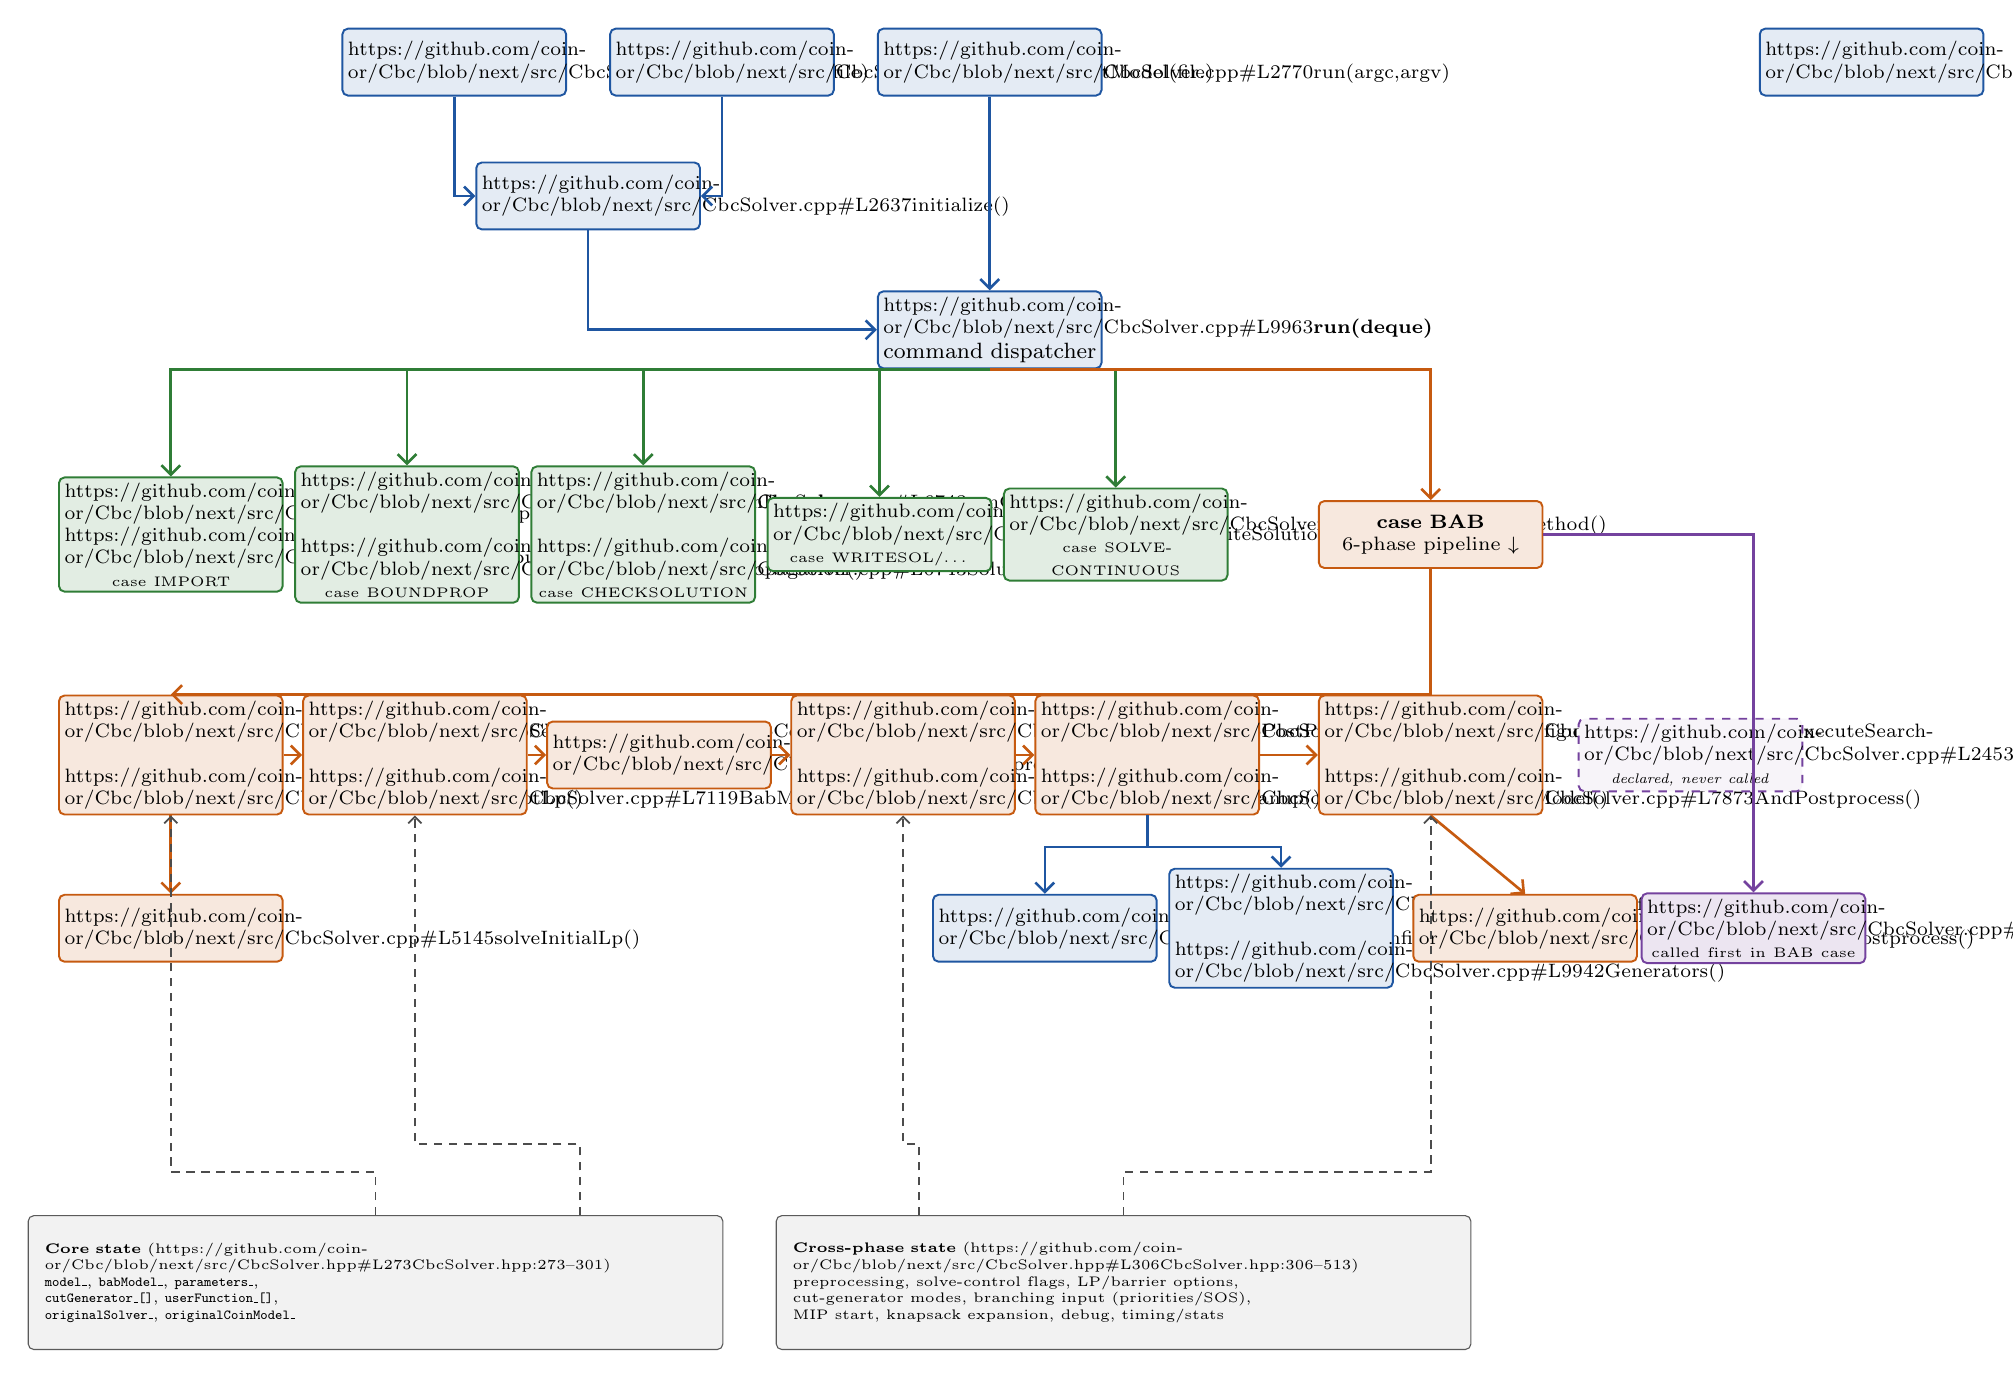
\begin{tikzpicture}[
    every node/.style={font=\scriptsize},
    box/.style={draw, rounded corners=2pt, align=center, text width=2.7cm,
                minimum height=0.85cm, inner sep=2pt, line width=0.7pt},
    api/.style={box, fill=capi!12, draw=capi},
    bab/.style={box, fill=cbab!14, draw=cbab},
    oth/.style={box, fill=cother!14, draw=cother},
    util/.style={box, fill=cutil!14, draw=cutil},
    orph/.style={box, fill=cutil!6, draw=cutil, dashed, text width=2.7cm},
    dat/.style={draw=cdata, fill=cdata!8, rounded corners=2pt, align=left, inner sep=6pt, font=\tiny},
    apiarr/.style={-{Straight Barb[scale=1.0]}, line width=0.95pt, capi},
    babarr/.style={-{Straight Barb[scale=1.0]}, line width=0.95pt, cbab},
    otharr/.style={-{Straight Barb[scale=1.0]}, line width=0.95pt, cother},
    utilarr/.style={-{Straight Barb[scale=1.0]}, line width=0.95pt, cutil},
    darr/.style={-{Straight Barb[scale=0.85]}, line width=0.65pt, cdata!85!black, dash pattern=on 3pt off 2.4pt}
  ]

  % ================= Row 0: convenience one-call wrappers =================
  \node[api] (solve)     at (-2.0, 16.6) {\ghc{2783}{solve(file)}};
  \node[api] (importpub) at (1.4, 16.6)  {\ghc{2801}{importModel(file)}};
  \node[api] (runargv)   at (4.8, 16.6) {\ghc{2770}{run(argc,argv)}};
  \node[api] (solveLp)   at (16.0, 16.6) {\ghc{2817}{solveLp(method)}};

  % ================= Row 1: initialize() + dispatcher hub =================
  \node[api] (initcall)  at (-0.3, 14.9) {\ghc{2637}{initialize()}};
  \node[api] (rundeque) at (4.8, 13.2) {\ghc{9963}{\textbf{run(deque)}}\\[1pt]\footnotesize command dispatcher};

  % ================= Row 2: dispatch fan-out (non-BAB actions) =================
  \node[oth] (imppriv)   at (-5.6, 10.6) {\ghc{2892}{importModel(}\\\ghc{2892}{inputQueue)}\\{\tiny case IMPORT}};
  \node[oth] (boundprop) at (-2.6, 10.6) {\ghc{6697}{runBound-}\\\ghc{6697}{Propagation()}\\{\tiny case BOUNDPROP}};
  \node[oth] (checksol)  at (0.4, 10.6) {\ghc{6743}{runCheck-}\\\ghc{6743}{Solution()}\\{\tiny case CHECKSOLUTION}};
  \node[oth] (writesol)  at (3.4, 10.6) {\ghc{5545}{writeSolution()}\\{\tiny case WRITESOL/\ldots}};
  \node[oth] (applylp)   at (6.4, 10.6) {\ghc{1117}{applyLpMethod()}\\{\tiny case SOLVECONTINUOUS}};
  \node[bab] (babcase)   at (10.4, 10.6) {\textbf{case BAB}\\ 6-phase pipeline $\downarrow$};

  % ================= Row 3: the 6-phase BAB pipeline (left to right chain) =================
  \node[bab] (setup)      at (-5.6, 7.8) {\ghc{6779}{babSetupAnd-}\\\ghc{6779}{RootLp()}};
  \node[bab] (cfgbab)     at (-2.5, 7.8) {\ghc{7119}{babConfigure-}\\\ghc{7119}{BabModel()}};
  \node[bab] (prep)       at (0.6, 7.8)  {\ghc{3191}{preprocess()}};
  \node[bab] (postpp)     at (3.7, 7.8)  {\ghc{7357}{babPostPreprocess-}\\\ghc{7357}{Cleanup()}};
  \node[bab] (cfgsearch)  at (6.8, 7.8)  {\ghc{7480}{babConfigure-}\\\ghc{7480}{SearchModel()}};
  \node[bab] (execsearch) at (10.4, 7.8) {\ghc{7873}{babExecuteSearch-}\\\ghc{7873}{AndPostprocess()}};

  % ================= Row 4: pipeline sub-calls =================
  \node[bab] (solveilp) at (-5.6, 5.6) {\ghc{5145}{solveInitialLp()}};
  \node[api] (cfgheur)  at (5.5, 5.6)  {\ghc{9936}{configureHeuristics()}};
  \node[api] (cfgcuts)  at (8.5, 5.6)  {\ghc{9942}{configureCut-}\\\ghc{9942}{Generators()}};
  \node[bab] (postp)    at (11.6, 5.6) {\ghc{4432}{postprocess()}};

  % ================= Row 5: bookkeeping helpers =================
  \node[util] (paramchg) at (14.5, 5.6) {\ghc{2597}{printParamChanges()}\\{\tiny called first in BAB case}};
  \node[orph] (reset)    at (13.7, 7.8) {\ghc{2453}{resetRunState()}\\{\tiny\itshape declared, never called}};

  % ================= Data / state panels (bottom band, spanning full width) =================
  \node[dat, text width=8.4cm, minimum height=1.7cm] (dataA) at (-3.0, 1.1) {
    \textbf{Core state} (\ghh{273}{CbcSolver.hpp:273--301})\\
    \texttt{model\_}, \texttt{babModel\_}, \texttt{parameters\_},\\
    \texttt{cutGenerator\_[]}, \texttt{userFunction\_[]},\\
    \texttt{originalSolver\_}, \texttt{originalCoinModel\_}
  };
  \node[dat, text width=8.4cm, minimum height=1.7cm] (dataB) at (6.5, 1.1) {
    \textbf{Cross-phase state} (\ghh{306}{CbcSolver.hpp:306--513})\\
    preprocessing, solve-control flags, LP/barrier options,\\
    cut-generator modes, branching input (priorities/SOS),\\
    MIP start, knapsack expansion, debug, timing/stats
  };

  % ================= Edges: convenience wrappers (blue = public API) =================
  \draw[apiarr] (solve.south) |- (initcall.west);
  \draw[apiarr] (importpub.south) |- (initcall.east);
  \draw[apiarr] (initcall.south) |- (rundeque.west);
  \draw[apiarr] (runargv.south) -- (rundeque.north);

  % ================= Edges: dispatcher fan-out =================
  \draw[otharr] (rundeque.south) -| (imppriv.north);
  \draw[otharr] (rundeque.south) -| (boundprop.north);
  \draw[otharr] (rundeque.south) -| (checksol.north);
  \draw[otharr] (rundeque.south) -| (writesol.north);
  \draw[otharr] (rundeque.south) -| (applylp.north);
  \draw[babarr] (rundeque.south) -| (babcase.north);

  % ================= Edges: BAB pipeline chain (orange = BAB pipeline) =================
  \draw[babarr] (babcase.south) |- (setup.north);
  \draw[babarr] (setup.east) -- (cfgbab.west);
  \draw[babarr] (cfgbab.east) -- (prep.west);
  \draw[babarr] (prep.east) -- (postpp.west);
  \draw[babarr] (postpp.east) -- (cfgsearch.west);
  \draw[babarr] (cfgsearch.east) -- (execsearch.west);

  % ================= Edges: pipeline sub-calls (directly below their caller, orthogonal) =================
  \draw[babarr] (setup.south) -- (solveilp.north);
  \draw[apiarr] (cfgsearch.south) -- ++(0,-0.4) -| (cfgheur.north);
  \draw[apiarr] (cfgsearch.south) -- ++(0,-0.4) -| (cfgcuts.north);
  \draw[babarr] (execsearch.south) -- (postp.north);

  % ================= Edges: bookkeeping (purple) =================
  \draw[utilarr] (babcase.east) -| (paramchg.north);

  % ================= Edges: data ownership (aggregated, dashed grey, non-crossing) =================
  \draw[darr] (dataA.north) -- ++(0,0.55) -| (setup.south);
  \draw[darr] (dataA.north) ++(2.6,0) -- ++(0,0.9) -| (cfgbab.south);
  \draw[darr] (dataB.north) ++(-2.6,0) -- ++(0,0.9) -| (postpp.south);
  \draw[darr] (dataB.north) -- ++(0,0.55) -| (execsearch.south);

\end{tikzpicture}%
}
\end{center}

\vspace{-3pt}
{\scriptsize\textit{Arrows show call/return relationships within the modularized \texttt{BAB} pipeline
(\S\ref{sec:pipeline}); dashed grey arrows indicate representative reads/writes of the shared state
panel on the left (most pipeline methods touch several state groups --- only the busiest links are
drawn to keep the diagram readable). All labels link to the corresponding line in
\texttt{coin-or/Cbc}, branch \texttt{next}.}}
\end{landscape}

\end{document}
